% !Mode:: "TeX:UTF-8"

\begin{frame}{第十八讲、重积分的计算}
	\linespread{1.5}
	\begin{enumerate}
	  \item {\bf 内容与要求}{\b (\S 11.2)}
	  \begin{itemize}
% 	    \item 理解二重积分和三重积分的概念
		\item 熟练掌握将二重积分化为累次积分加以计算的方法
	    \item 熟练掌握三重积分计算的微元法和截痕法
% 	    \item 熟练掌握将二重积分化为累次积分加以计算的方法
% 	    \item 了解最小二乘法
	  \vspace{1em}
	  \end{itemize}
	  \item {\bf  课后作业:}
	  \begin{itemize}
% 	    \item {\b 习题11.1:4,7(2),8(2)}
	    \item {\b 习题11.2:1(4),3(1,3),5(2,4),6(2,3)}
	    \item {\b 习题11.2:4(1,3),7(1,3),11}
	  \end{itemize}
	\end{enumerate}
\end{frame}

\section{二重积分的计算}

\begin{frame}{二重积分与累次积分}
	\linespread{1.2}\pause 
	{\bb 二重积分:}
	$$\alert{\iint_Df(x,y)\d\sigma=\lim_{d(T)\to
	  0}\sum_{i=1}^nf(\xi_i,\eta_i)\Delta\sigma_i}$$
	\pause 令$\d\sigma=\d y\d x$,\pause 且
	$$D=\{x_1\leq x\leq x_2,\varphi_1(x)\leq y\leq \varphi_2(x)\}$$
	\pause 则二重积分可化为{\bb 累次积分:}
	$$\alert{\iint_Df(x,y)\d\sigma=\int_{x_1}^{x_2}
	\int_{\varphi_1(x)}^{\varphi_2(x)}f(x,y)\d y\d x}$$
\end{frame}

\begin{frame}{积分区域与累次积分的次序}
	\linespread{1.2}\pause 
	\ba{将二重积分化为累次积分时,不同的积分次序,对应于不同的积分区域表示方法}\pause 
	\begin{exampleblock}{{\bf 例1}\hfill}
		计算
		$$\iint_Dxy\d\sigma,$$
		其中$D$为抛物线$y=x^2$和$x=y^2$所围区域。
	\end{exampleblock}\pause 
	\begin{itemize}
	  \item {\bb 先$x$后$y$:}$D:y^2\leq x\leq\sqrt y,\,0\leq y\leq 1$\pause 
	  \item {\bb 先$y$后$x$:}$D:x^2\leq y\leq\sqrt x,\,0\leq x\leq 1$
	\end{itemize}
\end{frame}

\begin{frame}{二重积分的计算}
	\linespread{1.2}\pause 
	\begin{enumerate}
	  \item {\bb 画图:}描绘积分区域$D$的图形\pause 
	  \item {\bb 定限:}确定累次积分的积分限\pause 
	  \item {\bb 求积分:}依次计算累次积分的值\pause 
	\end{enumerate}
	\begin{exampleblock}{{\bf 例2}\hfill}
		计算
		$$\iint_D\df{x^2}{y^2}\d\sigma,$$
		其中$D$由直线$y=2,\,y=x$和$xy=1$围成。
	\end{exampleblock}
\end{frame}

\begin{frame}
	\linespread{1.2}
	\begin{exampleblock}{{\bf 例3}\hfill}
		计算
		$$\iint_D\df{\sin y}{y}\d\sigma,$$
		其中$D$由$x=y^2$和$y=x$所围成。
	\end{exampleblock}
	\bigskip\pause 
	\ba{合理选择积分次序,简化累次积分的计算}
\end{frame}

% \begin{frame}
% 	\linespread{1.2}
% 	\begin{columns}
% 		\column{.5\textwidth}
% 			\begin{exampleblock}{{\bf 例7}\hfill}
% 			求两柱面
% 			$$x^2+y^2=R^2,$$
% 			$$x^2+z^2=R^2$$
% 			相交所围成的立体体积。
% 		\end{exampleblock}
% 		\column{.5\textwidth}
% 			\begin{center}
% 			\resizebox{!}{4.5cm}{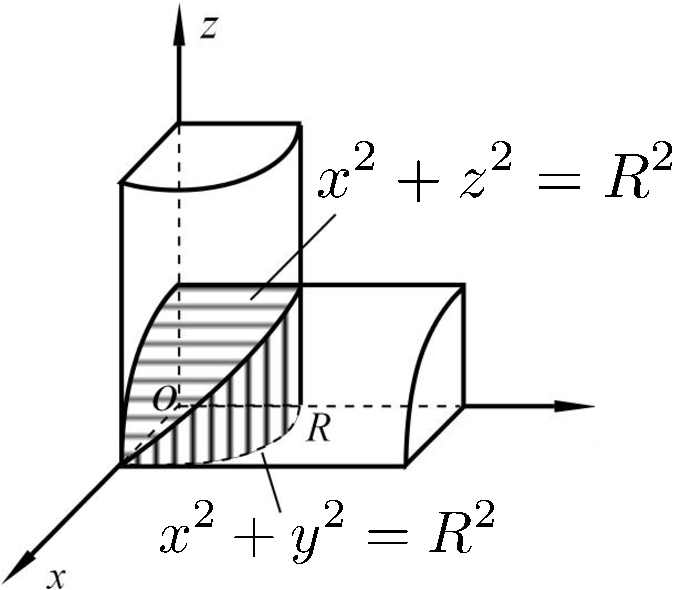
\includegraphics{./images/ch11/intersectV.pdf}}
% 		\end{center}
% 	\end{columns}
% \end{frame}

\begin{frame}
	\linespread{1.2}
	\begin{exampleblock}{{\bf 例4}\hfill}
		计算累次积分
		$$I=\int_{1/4}^{1/2}\int_{1/2}^{\sqrt y}e^{y/x}\d x\d y+
		\int_{1/2}^1\int_y^{\sqrt y}e^{y/x}\d x\d y$$
	\end{exampleblock}
\end{frame}

\begin{frame}
	\linespread{1.2}
% 	\begin{columns}
% 		\column{.5\textwidth}
			\begin{exampleblock}{{\bf 例5}\hfill}
			求两柱面$x^2+y^2=R^2,\, x^2+z^2=R^2$
			相交所围成的立体体积。
		\end{exampleblock}\pause 
% 		\column{.5\textwidth}
			\begin{center}
			\resizebox{!}{5cm}{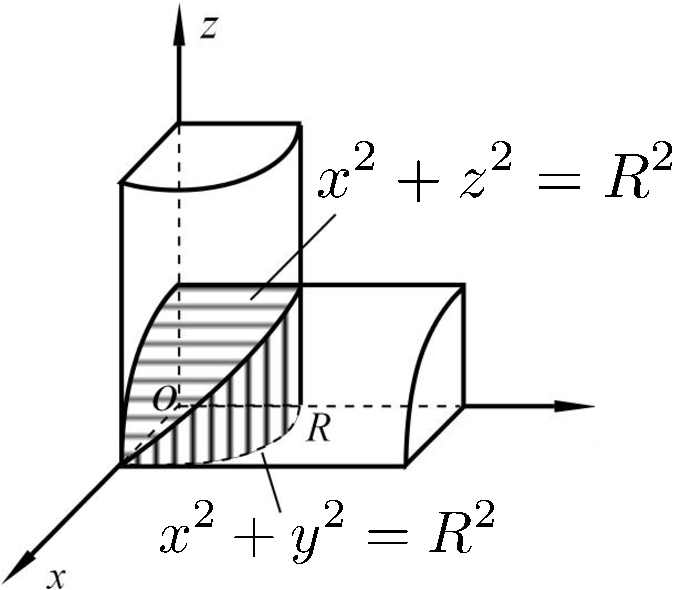
\includegraphics{./images/ch11/intersectV.pdf}}
		\end{center}
% 	\end{columns}
\end{frame}

\section{三重积分的计算}

\begin{frame}{三重积分的计算}
	\linespread{1.2}\pause 
	$$\alert{I=\iiint_{\Omega}f(x,y,z)\d V}$$
	\begin{enumerate}\pause 
	  \item {\bb 微元法:}
	  $$I=\iint_D\int_{z_1(x,y)}^{z_2(x,y)}f(x,y,z)\d z\d\sigma$$\pause 
	  \item {\bb 截面法:}
	  $$I=\int_{z_1}^{z_2}\iint_{D(z)}f(x,y,z)\d\sigma \d z$$
	\end{enumerate}
\end{frame}

\begin{frame}{1、微元法}
	\linespread{1.2}
	\begin{columns}
		\column{.5\textwidth}
			设$\Omega$在$xOy$平面上的投影区域为$D$,\pause $\d V=\d z\d\sigma$,\pause 
			$$\Omega=\{z_1(x,y)\leq z\leq z_2(x,y),$$
			$$\quad (x,y)\in D\}$$
		\column{.5\textwidth}
			\begin{center}
				\pause \resizebox{!}{4.5cm}{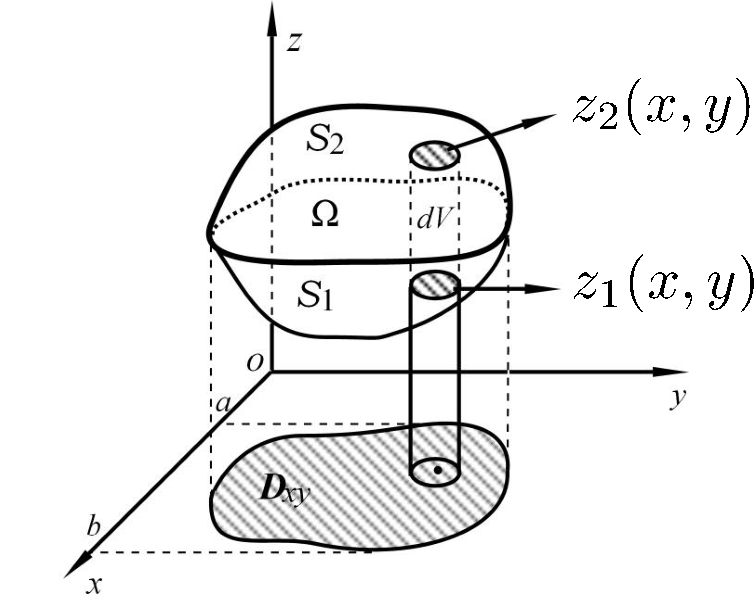
\includegraphics{./images/ch11/DxyZ.pdf}}\pause 
			\end{center}
	\end{columns}
	$$\alert{I=\iiint_{\Omega}f(x,y,z)\d
	V=\iint_D\int_{z_1(x,y)}^{z_2(x,y)}f(x,y,z)\d z\d\sigma}$$
\end{frame}

\begin{frame}
	\linespread{1.2}
	$$\alert{I=\iiint_{\Omega}f(x,y,z)\d
	V=\iint_D\int_{z_1(x,y)}^{z_2(x,y)}f(x,y,z)\d z\d\sigma}$$
	\pause 
	\begin{exampleblock}{{\bf 例6}\hfill}
		计算三重积分
		$$I=\iiint_{\Omega}\df 1{(1+x+y+z)^3}\d V,$$
		其中$\Omega$为平面$x+y+z=1$与三个坐标面所围成的空间区域。
	\end{exampleblock}
\end{frame}

\begin{frame}{2、截面(痕)法}
	\linespread{1.2}
	\begin{columns}
		\column{.52\textwidth}
			取$\Omega$的水平截面,\pause 其在$xOy$平面上的投影区域为$D(z)$,
			\pause $\d V=\d\sigma \d z$,\pause 
			$$\Omega=\{(x,y)\in D(z),z_1\leq z\leq z_2\}$$
% 			$$\quad \}$$
		\column{.48\textwidth}
			\begin{center}
				\pause \resizebox{!}{4.5cm}{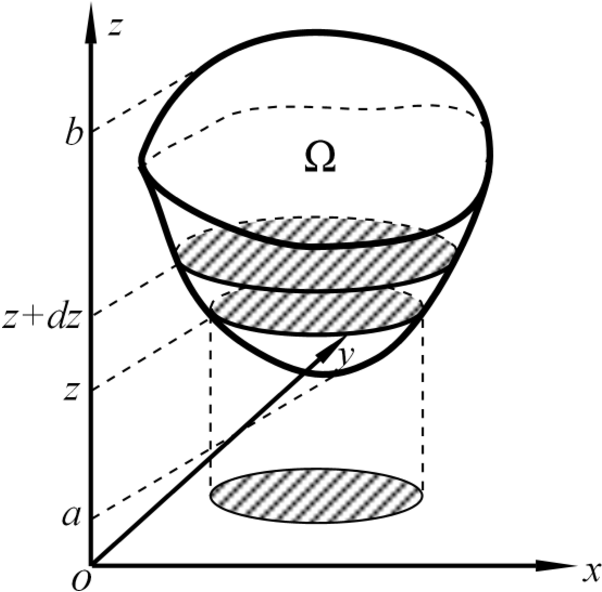
\includegraphics{./images/ch11/Dzxy.pdf}}\pause 
			\end{center}
	\end{columns}
	$$\alert{I=\iiint_{\Omega}f(x,y,z)\d
	V=\int_{z_1}^{z_2}\iint_{D(z)}f(x,y,z)\d\sigma \d z}$$
\end{frame}

\begin{frame}
	\linespread{1.2}
	$$\alert{I=\iiint_{\Omega}f(x,y,z)\d
	V=\int_{z_1}^{z_2}\iint_{D(z)}f(x,y,z)\d\sigma \d z}$$\pause 
	\begin{exampleblock}{{\bf 例7}\hfill}
		计算三重积分
		$$I=\iiint_{\Omega}z^2\d V,$$
		其中$\Omega:\df{x^2}{a^2}+\df{y^2}{b^2}+\df{z^2}{c^2}\leq 1$。
	\end{exampleblock}
\end{frame}

\begin{frame}
	\linespread{1.2}
	\begin{exampleblock}{{\bf 例8}\hfill}
		将三重积分
		$$I=\iiint_{\Omega}f(x,y,z)\d V,$$
		化为累次积分,其中$\Omega$为曲面$z=1-x,y=1-z^2$及三个坐标平面所围空间闭区域。
	\end{exampleblock}
\end{frame}

\begin{frame}
	\linespread{1.2}
	\begin{exampleblock}{{\bf 例9}\hfill}
		计算三重积分
		$$I=\iiint_{\Omega}(x+y+2z)\d V,$$
		其中$\Omega$为球体$x^2+y^2+z^2\leq R^2\,(R>0)$在第一卦限中的部分。
	\end{exampleblock}
\end{frame}

\begin{frame}[<+->]{小结}
	\linespread{1.2}
	\begin{enumerate}
% 	  \item {\bf 重积分的定义:}“分割取近似,做和求极限”
% 	  $$\iint_Df(x,y)d\sigma=\lim_{d(T)\to
% 		  0}\sum_{i=1}^nf(\xi_i,\eta_i)\Delta\sigma_i$$
% 	  \item {\bf 重积分的基本性质}
% 	  \begin{itemize}
% 	    \item 与定积分的性质加以类比
% 	  \end{itemize}
	  \item {\bf 二重积分的计算}
	  $$\iint_Df(x,y)\d\sigma=\int_{x_1}^{x_2}
	\int_{\varphi_1(x)}^{\varphi_2(x)}f(x,y)\d y\d x$$
	  \item {\bf 三重积分的计算}
	  \begin{itemize}
	    \item {微元法{\bb (2+1)}:}先投影,再定$z$
% 	    $$I=\iint_D\int_{z_1(x,y)}^{z_2(x,y)}f(x,y,z)dzd\sigma$$
	    \item {截面法{\bb (1+2)}:}先定$z$,再投影
% 	    $$I=\int_{z_1}^{z_2}\iint_{D(z)}f(x,y,z)d\sigma dz$$
	  \end{itemize}
	\end{enumerate}
	\pause
	\hrule
	\bigskip \pause 
	\begin{center}
		\ba{基本步骤:画图$\to$定限$\to$积分}\pause
		
		\ba{关键点:积分次序与积分区域的表示}
	\end{center}
	
\end{frame}

%=====================================
 
% \begin{frame}{title}
% 	\linespread{1.2}
% 	\begin{exampleblock}{{\bf title}\hfill}
% 		123
% 	\end{exampleblock}
% \end{frame}
% 
% \begin{frame}{title}
% 	\linespread{1.2}
% 	\begin{block}{{\bf title}\hfill}
% 		123
% 	\end{block}
% \end{frame}